\section{Class-III and Class-IV: staging births}
\label{sec:class-iii-iv}

In Class-III and Class-IV the birth does more than form structure. Its location depends on the observation timescale, and it does so in both structural channels, so staging becomes part of the class identity. Class-III has no drive; Class-IV adds drive. These classes are harder to establish than Class-I and Class-II, and their claims are tied to the manual lens.

\paragraph{Representatives.} Both representatives come from the replicated-portal family described before Proposition~\ref{prop:lumpability}. They use fast weight $1.0$, fast--portal weight $0.02$, portal--cross weight $1.2$, and portal-self weight $4.0$. The Class-III kernel (\texttt{replicated\_portal\_sp4}) is this symmetric kernel. The Class-IV kernel (\texttt{replicated\_portal\_sp4\_drive\_f}) mixes it, with weight $0.12$, with a biased ring on all $N$ states (stay, forward, and backward weights $0.10$, $0.57$, and $0.33$). Both are analysed with the manual two-block lens on a 18-point grid from $\lambda=0.05$ to $1$.

\paragraph{Readings.} Table~\ref{tab:class-iii-iv-summary} gives the readings at $N=64$, the size used for the common map. Figure~\ref{fig:structural-curves} (last two columns) shows the curves. In both classes the closure and objecthood boundaries move by more than $0.15$ between $\tau=1$ and $\tau=2$, so $P4_{\mathrm{dual}}$ exceeds the strict threshold: $0.202$ for Class-III and $0.216$ for Class-IV. Class-III has exactly zero affinity. Class-IV has $\mathrm{Aff}_{\mathrm{ref}}=2.99\times10^{-3}$, with exact lower bound $2.96\times10^{-3}$.

\begin{table}[tbp]
\centering
\small
\caption{Class-III and Class-IV readings at $N=64$ (manual lens). Both have packaging and staging on.}
\label{tab:class-iii-iv-summary}
\setlength{\tabcolsep}{5pt}
\begin{tabular}{@{}llccccc@{}}
\toprule
Class & $P6_{\mathrm{drive}}$
  & $\lambda_{\mathrm{CE}}$
  & $\lambda_{M_{\mathrm{obj}}}$
  & $\lambda_{\mathrm{struct,ref}}$
  & $\mathrm{Aff}_{\mathrm{ref}}$
  & $P4_{\mathrm{dual}}$ \\
\midrule
III & off & 0.562 & 0.123 & 0.562 & $0$ (exact)          & 0.202 \\
IV  & on  & 0.533 & 0.067 & 0.533 & $2.99\times 10^{-3}$ & 0.216 \\
\bottomrule
\end{tabular}
\end{table}

\paragraph{Persistence across sizes.} Both labels hold at $N=16$, $32$, $64$, and $128$, and each of these points is certified exactly (Table~\ref{tab:certificates}). For Class-III, Proposition~\ref{prop:lumpability} gives more: the readings are identical at every admissible size $N=8m\ge16$, because the dynamics lumps exactly onto four state types. For Class-IV the readings drift with size. The structural boundary moves from $0.607$ to $0.518$, the affinity lower bound grows from $1.6\times10^{-3}$ to $3.6\times10^{-3}$, and $P4_{\mathrm{dual}}$ grows from $0.183$ to $0.222$. The label is unchanged, but we make no claim beyond $N=128$. At $N=128$ the Class-IV objecthood boundary is left-censored at the first grid point. The label is unaffected because the structural reference is set by the resolved closure boundary.

\paragraph{Why the two-level staging rule matters here.} The Class-I and Class-II representatives also show timescale sensitivity (Section~\ref{sec:class-i-ii}). What sets Class-III and Class-IV apart is that the shift is large in \emph{both} channels at once. Without the strict rule, any system with a moderate one-channel shift would be counted as a staging birth. With it, and in the absence of a boundary appearing or disappearing between timescales, staging becomes a class label only when the closure and objecthood descriptions both move with the timescale.

\paragraph{Shadow ensembles.} To see whether the staging classes support more than a yes/no label, we perturbed each representative's three portal weights by $\pm5\%$, one at a time. For Class-IV the four drive parameters are perturbed by $\pm5\%$ as well. We kept only perturbations that preserve the label at all four sizes. Every candidate passed, so the ensembles have 7 members (Class-III) and 15 members (Class-IV), counting the unperturbed kernel, at each of 18 values of $\lambda$ and each size. On these ensembles we compute the susceptibility $\chi=N\,\mathrm{Var}(\Delta M_{\mathrm{obj}})$ of the timescale difference $\Delta M_{\mathrm{obj}}=M_{\mathrm{obj}}(\tau{=}2)-M_{\mathrm{obj}}(\tau{=}1)$, together with a Binder-type moment ratio \cite{fisher_barber_1972,binder_1981_prl}.

Figure~\ref{fig:shadow-susceptibility} shows the result. The susceptibility peaks near $\lambda\approx0.4$--$0.5$, with peak values from $1.3\times10^{-5}$ ($N=16$) to $1.0\times10^{-4}$ ($N=128$) for Class-III and from $4.9\times10^{-6}$ to $4.8\times10^{-5}$ for Class-IV. These numbers must be read with care. The ensemble is a distribution over perturbed parameters, not a thermodynamic ensemble. For Class-III the distribution of $\Delta M_{\mathrm{obj}}$ is exactly the same at every size (Proposition~\ref{prop:lumpability}), so $\chi$ grows exactly in proportion to $N$, because of the factor $N$ in its definition, and not because of any critical behaviour. For Class-IV the peak value of $\chi/N$ rises only slowly, by about $21\%$ from $N=16$ to $128$, although at the smallest $\lambda$ the relative increase is larger. The Binder-type ratio is within $0.01$ of $2/3$ at every point except $\lambda=1$, where all members coincide and the ratio is undefined. The value $2/3$ is what one expects for a narrow distribution centred away from zero. The panels are therefore a usable description of how $\Delta M_{\mathrm{obj}}$ fluctuates within a class, but they provide no evidence for critical exponents.

\begin{figure}[tbp]
\centering
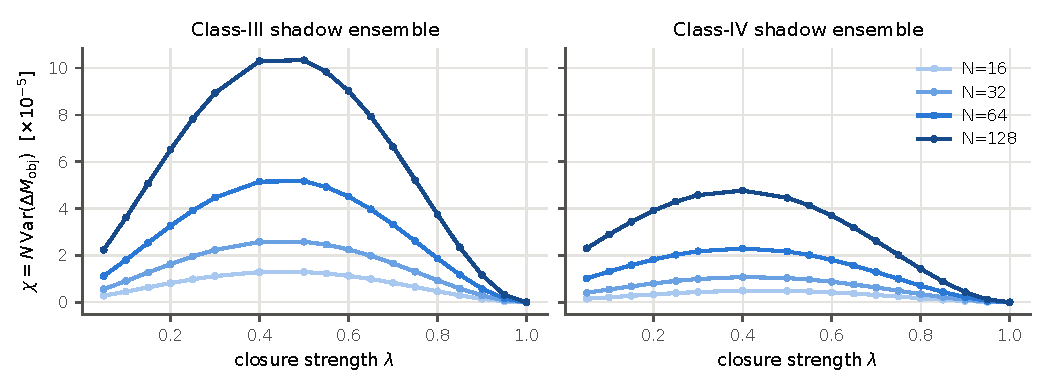
\includegraphics[width=\textwidth]{figures/shadow_susceptibility.pdf}
\caption{Shadow-ensemble susceptibility of the timescale difference $\Delta M_{\mathrm{obj}}$ under small class-preserving perturbations (manual lens). For Class-III the underlying distribution does not depend on $N$, so the curves differ only by the factor $N$ in $\chi$. For Class-IV, $\chi/N$ grows slightly with $N$. These are perturbation ensembles, not thermodynamic ones, and are not used for exponent claims.}
\label{fig:shadow-susceptibility}
\end{figure}

\paragraph{Lens dependence.} Replacing the manual lens with either automatic lens removes the staging label (Table~\ref{tab:class-iii-iv-lens-caveat}). The two automatic lenses give identical readings here. For Class-III they still find structure and no drive, so the birth is relabelled Class-I at both tested sizes. For Class-IV the result is worse. At $N=32$ the drive reading at the shifted boundary falls between the off and on thresholds, so drive is unknown and the system is unclassified. At $N=128$ drive is on but the objecthood shift vanishes, giving Class-II. In both classes the automatic lenses lose staging \emph{activation}, which is the defining feature. Class-III loses even the weak $P4$-like signal. Class-IV keeps a $P4$-like signal, because one of its shifts still exceeds $0.05$, but never both shifts above $0.15$.

\begin{table}[tbp]
\centering
\small
\caption{Class-III and Class-IV representatives under the two automatic lenses (spectral sign-pattern and diffusion-quantile; their readings coincide). The manual-lens label is confirmed at both sizes.}
\label{tab:class-iii-iv-lens-caveat}
\setlength{\tabcolsep}{4pt}
\begin{tabularx}{\linewidth}{@{}l c l l l Y@{}}
\toprule
Representative & $N$ & Manual & Automatic & $P5$ / $P6_{\mathrm{drive}}$ & Staging \\
\midrule
Class-III & 32  & Class-III & Class-I      & on / off     & no shift in either channel \\
Class-III & 128 & Class-III & Class-I      & on / off     & no shift in either channel \\
Class-IV  & 32  & Class-IV  & unclassified & on / unknown & shifts $0.119$, $0.232$: one below $0.15$ \\
Class-IV  & 128 & Class-IV  & Class-II     & on / on      & objecthood shift $0$ \\
\bottomrule
\end{tabularx}
\end{table}

\paragraph{What is established.} In the manual-lens channel, staging births exist with and without drive. They are certified exactly at four sizes and, for Class-III, at every admissible size, and they are separated from each other and from Class-I and Class-II by the measured observables. What is not established is that these labels survive an arbitrary change of coarse-graining. The two automatic lenses we tested do not reproduce them. Section~\ref{sec:discussion} returns to what this does and does not imply.
